
\chapter{Prédicteurs et résultats}

\section{Comparaison des modèles mis en place}

Les modèles présentés ci-dessous ont été testés en cross validation 10 fold parmi les algorithmes suivants : 
Random Forest, Gradient Boosting avec XGBoost, Multilayer Perceptron, KNN.
Les paramètres de ces algorithmes ont été dans un premier temps testées pour quelques valeurs standards (exemple:
$n\_estimator$ = 100 ou 200 pour un random forest)
Si les performances en cross validation étaient similaires entre les différents algorithmes
testés, nous utilisions alors un GridSearchCV pour optimiser les paramètres des modèles et
déterminer le meilleur. 
Si au contraire un modèle était d'emblée au dessus des autres en termes de performances, 
seul cet algorithme était alors optimisé avec GridSearchCV (les temps d'exécution étant
relativement longs).

\textbf{1-} Le premier modèle mis en place avait pour but d'éviter la surcharge de variables et de 
synthétiser l'information dans des variables plus parcimonieuses. C'est dans ce but que les 
variables BUYER_REGION et SELLER_REGION ont été créées à la place de BUYER_DEPARTMENT et
SELLER_DEPARTMENT. Par exemple, la variable BUYING_DATE avait été synthétisée en seulement
3 groupes significatifs représentant les 3 périodes de l'année où les pourcentages de 
réclamations et le nombre de ces réclamations étaient similaires. De même, la variable
PRODUCT_TYPE qui possède 137 niveaux n'avait été restreinte qu'aux types ayant un impact visible
sur le type de réclamation. 

AUC : 0,57

algorithme : random forest (n_estimators=100).

\textbf{2-} Le deuxième modèle mis en place a consisté cette fois-ci à garder le plus d'information
possible quitte à risquer d'avoir un peu de sur-apprentissage. Nous avons ainsi à la fois 
gardé les informations liées aux départements mais aussi celles liées aux régions et 
transformé l'ensemble des niveaux de la variable PRODUCT_TYPE en variables binaires.

AUC : 0,60

algorithme : random forest (n_estimators=100)

\begin{center}
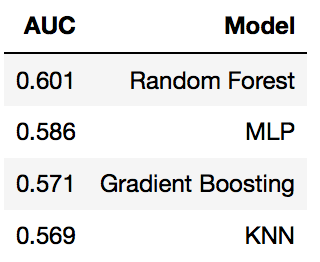
\includegraphics[scale=0.5]{assets/auc1} 
\end{center}

\textbf{3-} L'avancée majeure de notre modèle vient avec cette troisième phase où nous avons
tenter de prédire dans un premier temps la présence ou l'absence de réclamation et le cas 
échéant, prédire le type de réclamation avec un second modèle entrainé uniquement sur les
données où une réclamation a été portée. Les variables restent les mêmes qu'au modèle
précédent. La motivation derrière ce changement est que la classe '-' représente 50\%
de l'effectif total et correspond aussi au cas singulier de l'absence de réclamation, 
alors que les autres labels correspondent à un type de réclamation.
C'est avec cette amélioration que nous nous sommes hissés dans le top 10 du classement.

AUC : 0,63

algorithme de prédiction claim/no claim : random forest (n_estimators=200). \\
algorithme de prédiction du type de claim : random forest (n_estimators=100).

\textbf{4-} Une étape importante a ensuite été de modifier l'encodage du vecteur des
réclamations qui était jusqu'à présent encodé avec un labelBinarizer qui est typiquement utilisé
dans les problèmes de classification multiclasses pour obtenir des variables binaires.
Nous avons utilisé ici un encodage différent en associant un entier à chaque type de
réclamation, classées par ordre de fréquence d'apparition dans le jeu de donné : 0 lorsqu'il
n'y a pas de réclamation jusqu'à 7 pour FAKE. Cet encodage a apporté un gain non négligeable
dans notre score avec les mêmes algorithmes.

AUC : 0,64

algorithme de prédiction claim/no claim : random forest (n_estimators=200). \\
algorithme de prédiction du type de claim : random forest (n_estimators=100).

\begin{center}
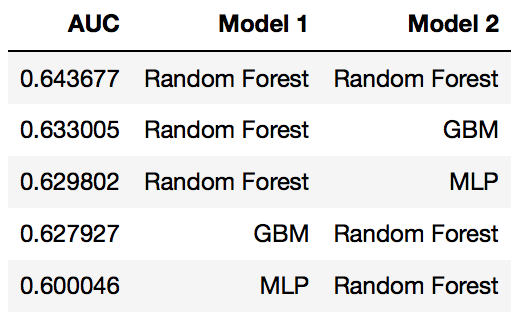
\includegraphics[scale=0.5]{assets/auc2} 
\end{center}

\textbf{5-} Les dernières modifications apportées à notre modèle résident dans la création
des features liés aux distances relatives entre acheteur et vendeur SELLER_BUYER_REGION_DISTANCE 
et SELLER_COUNTRY_DISTANCE. 

AUC : 0,649

algorithme de prédiction claim/no claim : random forest (n_estimators=200). \\
algorithme de prédiction du type de claim : random forest (n_estimators=100).

Avec cette dernière modification nous avons alors atteint la 2nde place du classement,
le premier groupe ayant un score de 0,650 à cet instant.

\section{Analyse des résultats}

Nous pouvons noter que l'algorithme de random forest s'est toujours avéré le plus efficace
dans tous les types de modèles testés.

Parmi les paramètres testés avec GridSearchCV seul le paramètre n_estimators semble 
déterminant pour notre problème, les autres paramètres étant systématiquement optimisés
avec leur valeur par défaut :

\begin{itemize}
\item max_features='auto'
\item criterion='Gini'
\item max_depth=None
\end{itemize}

Un des changements déterminants dans l'amélioration de notre score a été le passage d'un
modèle de prédiction simple à un modèle en deux temps, avec un premier algorithme
de classification binaire claim/no claim. Nous pouvons observer avec les matrices de confusion
ci-dessous la différence majeure qui réside dans ce changement de méthode.

\vspace{4.5cm}
\textbf{Matrice de confusion du modèle 2:}
\vspace{0.5cm}
\begin{center}
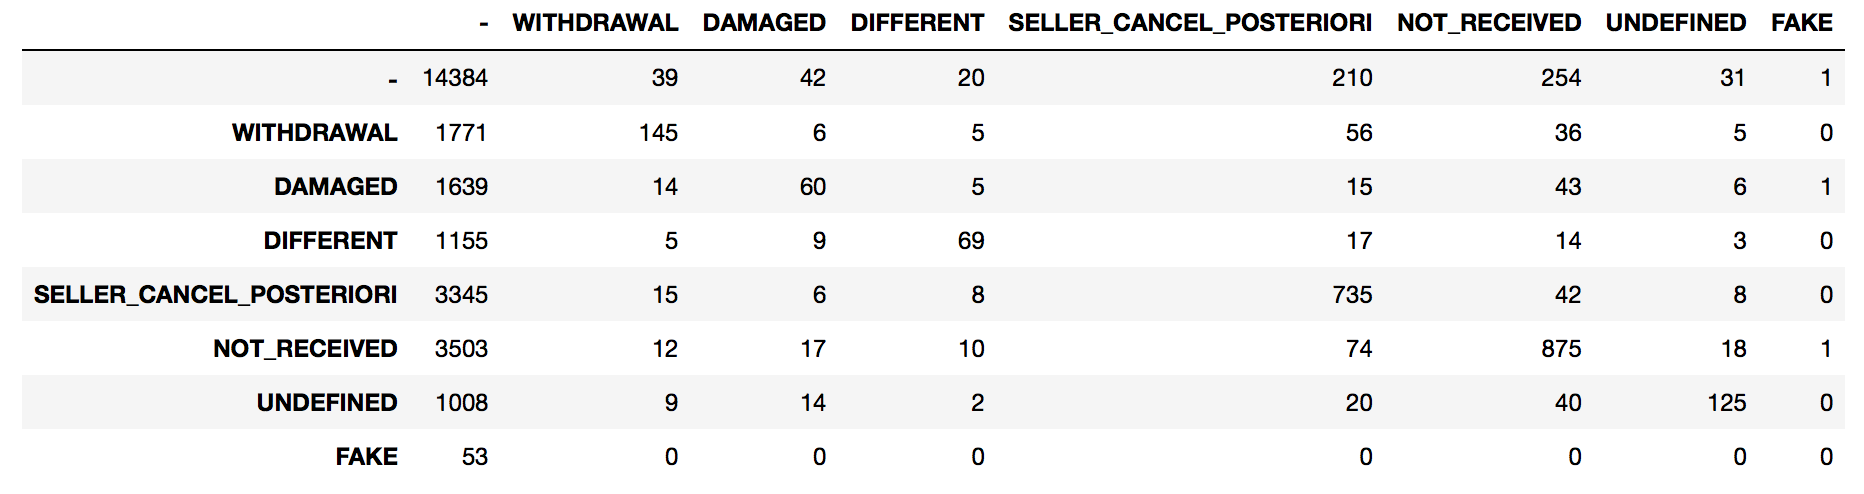
\includegraphics[scale=0.5]{assets/confmat1} 
\end{center}
\vspace{1.5cm}

\textbf{Matrice de confusion du modèle 3:}
\vspace{0.5cm}
\begin{center}
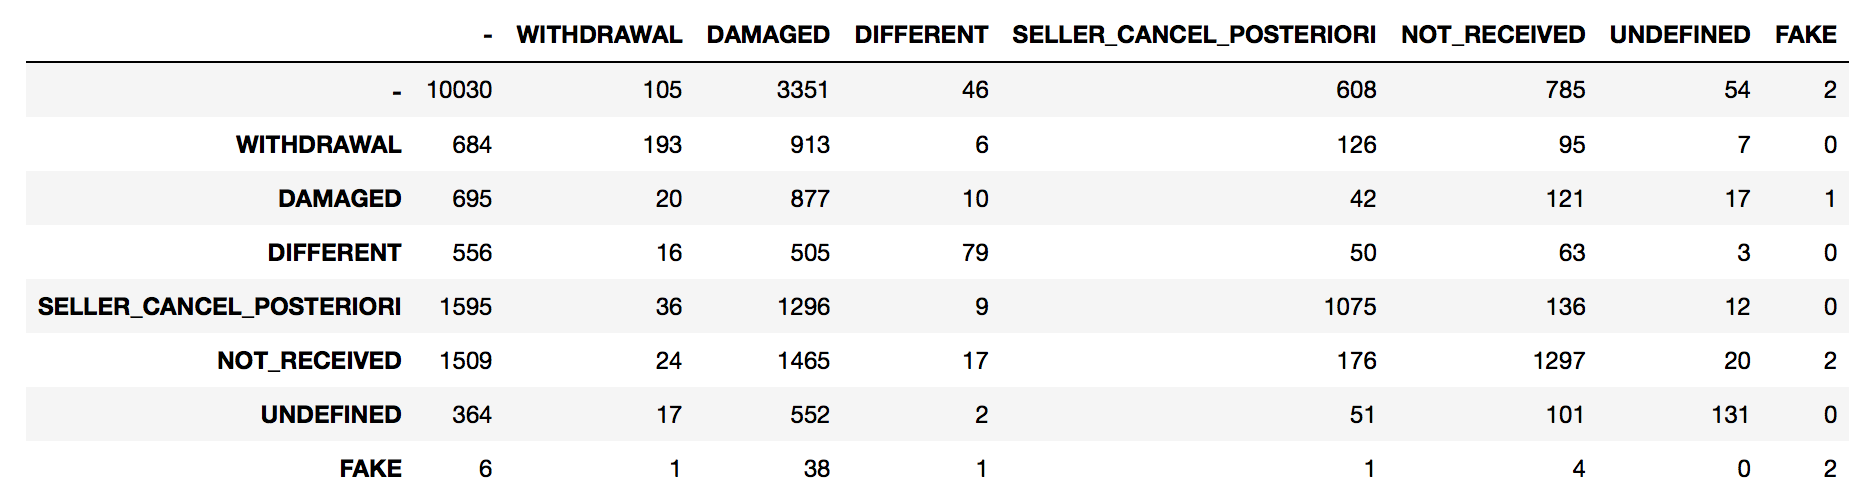
\includegraphics[scale=0.5]{assets/confmat2} 
\end{center}
\vspace{0.5cm}

En effet ce changement réside dans le fait que le modèle 2 a plus tendance a prédire qu'il
n'y aura pas de réclamation (biais conservateur) alors que le modèle 3 au contraire est plus 
susceptible de prédire qu'il y a réclamation (biais libéral). Le modèle 2 prédit 
majoritairement '-' qui est la classe majoritaire mais reste tout de même performant
sur les autres classes. En effet, en dehors des prédictions '-' le modèle 2 prédit 
majoritairement les bons types de réclamations. Cependant, le modèle 3 qui "prend plus de 
risque" est plus performant car il prédit mieux chacun des types de réclamations.

